\chapter{Obiettivi clinici dello studio della composizione del corpo}\label{capitolo2}
La TC, soprattutto nella regione addominale, è una tipologia di indagine molto diffusa per un’ampissima gamma di situazioni. Oltre allo scopo principale per cui una TC viene prescritta, che varia a seconda del caso, questa può essere utilizzata per ottenere una grande quantità di informazioni aggiuntive su fattori di rischio o altre patologie: l’approccio per cui vengono processate anche queste informazioni secondarie è chiamato di \textit{screening} opportunistico. Nel presente capitolo vengono presentati i vantaggi di questo approccio sotto diversi punti di vista, mediante alcuni studi che evidenziano la parziale inadeguatezza dei protocolli attualmente utilizzati in fase di valutazione della composizione corporea dei pazienti.

\section{Osteoporosi}
Uno degli obiettivi che può essere perseguito con lo \textit{screening} opportunistico è la valutazione della densità ossea, che se diventa troppo bassa configura una condizione clinica nota come osteoporosi, molto diffusa fra i pazienti, soprattutto donne, in età avanzata. L’età rappresenta infatti il maggior fattore di rischio, che però può essere contrastato riducendo altri fattori di rischio, come fumo di sigaretta, abuso di alcol e dieta carente di minerali essenziali. Se si scopre una densità ossea troppo bassa a seguito di uno \textit{screening} è possibile intervenire per tempo per evitare o ritardare l’insorgenza della malattia. La tecnica ad oggi più utilizzata per stimare la densità delle ossa è la densitometria ossea a raggi X a doppia energia, abbreviata in DXA: questa tecnica comporta la misurazione dell'attenuazione di due fasci di raggi X di diversa energia, in modo da poter derivare la densità (per unità di superficie, trattandosi di un'indagine che fornisce immagini bidimensionali) di un materiale in presenza di un altro a partire dalle diverse attenuazioni dei due materiali per energie diverse. Una volta nota l'attenuazione, possiamo risolvere un sistema di due equazioni a due incognite, approssimando l’attenuazione reale come quella di un fascio monocromatico attraverso la legge di Lambert-Beer (\eqref{lambert}), la quale può essere riscritta nel seguente modo:
\begin{equation}
    I = I_0\,\mathrm{e}^{-\mu x} = I_0\,\mathrm{e}^{-\left(\frac{\mu}{\rho}\right) \rho x} = I_0\,\mathrm{e}^{-\left(\frac{\mu}{\rho}\right) \sigma}\,,
\end{equation}
dove $\frac{\mu}{\rho}$ rappresenta il coefficiente di attenuazione di massa, i cui valori sono tabulati e dipendono dal materiale e dall'energia del fascio, e $\sigma$ è la densità di massa superficiale. Le due equazioni per i due fasci a energia differente sono:
    \[
\begin{sistema} 
I^\mathrm{L} = I_0\,\mathrm{e}^{- \left[ \left(\frac{\mu}{\rho}\right)^\mathrm{L}_\mathrm{s} \sigma_\mathrm{s} + \left(\frac{\mu}{\rho}\right)^\mathrm{L}_\mathrm{b} \sigma_\mathrm{b} \right]} \\
I^\mathrm{H} = I_0\,\mathrm{e}^{- \left[ \left(\frac{\mu}{\rho}\right)^\mathrm{H}_\mathrm{s} \sigma_\mathrm{s} + \left(\frac{\mu}{\rho}\right)^\mathrm{H}_\mathrm{b} \sigma_\mathrm{b} \right]}
\end{sistema}\,,
    \]
dove gli apici H e L indicano l'energia (alta o bassa) del fascio, mentre pedici s e b indicano il tipo di tessuto (molle o osseo). Il sistema è risolto per:
\begin{equation}
    \sigma_\mathrm{b} = \dfrac{R_\mathrm{s} \ln{\left(\dfrac{I}{I_0}\right)^\mathrm{H}}- \ln{\left(\dfrac{I}{I_0}\right)^\mathrm{L}}}{\left(\dfrac{\mu}{\rho}\right)^\mathrm{L}_\mathrm{b} - \left(\dfrac{\mu}{\rho}\right)^\mathrm{H}_\mathrm{b} R_\mathrm{s}}\,,
\end{equation}
dove con $R_\mathrm{s}$ indichiamo:
\begin{equation}
    R_\mathrm{s} = \dfrac{\left(\dfrac{\mu}{\rho}\right)^\mathrm{L}_\mathrm{s}}{\left(\dfrac{\mu}{\rho}\right)^\mathrm{H}_\mathrm{s}}\,.
\end{equation}
$\sigma_\mathrm{s}$ si trova esattamente allo stesso modo \cite[17-22]{iaea}. Nell'ambito della DXA, l'esame si effettua sul segmento lombare della colonna vertebrale, sul femore o sul polso, a seconda dell'età e del sesso del paziente. La densità ossea misurata viene confrontata col valore medio di una popolazione di giovani adulti sani, calcolando lo scostamento dal valore di riferimento in termini di deviazioni standard; il numero di deviazioni standard dal riferimento è definito \textit{T-score}. In presenza di un \textit{T-score} maggiore di $-1$ la densità ossea è considerata normale, tra $-1$ e $-2,5$ si configura l'osteopenia, mentre per \textit{T-score} inferiori a $-2,5$ viene diagnosticata l'osteoporosi \cite{siommms}.

Alternativamente, il calcolo della densità ossea può anche essere eseguito con una tecnica nota come TC quantitativa (QCT), ponendo vicino al paziente un fantoccio di fosfato di potassio (\figref{fig:fantoccio}), usato come riferimento per effettuare confronti tra la densità delle ossa del paziente e quella del fantoccio stesso \cite{Murray2017}. Il confronto viene effettuato attraverso la scala Hounsfield, che quantifica il valore di grigio dei pixel in un’immagine radiografica in unità di Hounsfield (HU), definite come segue:

\begin{equation}
    \mathrm{HU}(x,y,z) = 1000\times\frac{\mu(x,y,z) - \upmu_\mathrm{w}}{\upmu_\mathrm{w} - \upmu_\mathrm{a}}\,,
\end{equation}
dove $\mu(x,y,z)$ è il coefficiente di attenuazione lineare medio per elemento di volume (voxel) di tessuto in posizione $(x,y,z)$, mentre $\upmu_\mathrm{w}$ e $\upmu_\mathrm{a}$ sono i coefficienti di attenuazione lineare rispettivamente dell'acqua e dell'aria. Per l’acqua HU si annulla, per l’aria, che ha coefficiente di attenuazione lineare circa uguale a 1, assume il valore $-1000$; per quanto riguarda i tessuti del corpo, si va da un intervallo compreso tra $-80$ e $-30$\,HU per la maggior parte dei tessuti adiposi a un massimo di 3095\,HU per le ossa nella maggior parte dei macchinari di TC \cite[324-325]{bushberg}. La scala Hounsfield è importante perché stabilisce un criterio univoco di quantificazione per i valori di intensità dei pixel dell'immagine, permettendo così di confrontare immagini acquisite da macchinari diversi.
\begin{figure}[htp]
\centering
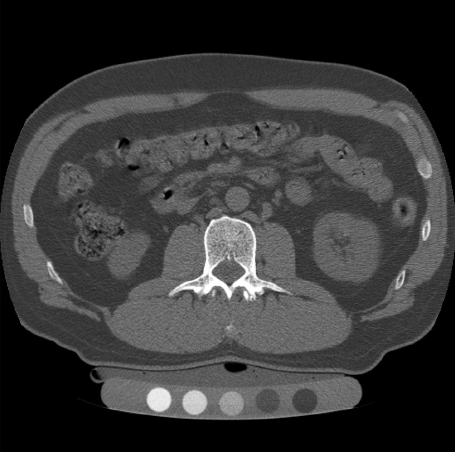
\includegraphics[scale=0.6505]{Immagini/fantoccio.png}\quad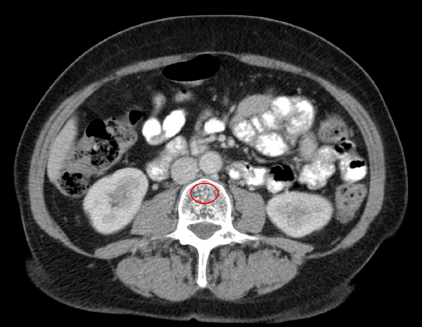
\includegraphics[scale=0.9]{Immagini/osteoporosi.png}
\caption{\label{fig:fantoccio} \textit{QCT eseguita con l'utilizzo di un fantoccio a diverse concentrazioni (immagine di sinistra) e CT addominale (L3), dove la vertebra presenta un valore di $106\,\mathrm{HU}$, compatibile con la diagnosi di osteoporosi (immagine di destra). Fonte:} \cite{wiki:fantoccio, Murray2017}.}
\end{figure}

Tornando alla QCT, questa ha un importante vantaggio rispetto alla DXA: trattandosi di un'indagine tomografica, questa misura la densità per unità di volume, al contrario delle misure della DXA che sono superficiali, ottenendo così dati riferiti al vero volume delle ossa. Valori di densità superiori ai $120\,\mathrm{mg}/\mathrm{cm}^3$ sono considerati normali, valori compresi tra 80 e $120\,\mathrm{mg}/\mathrm{cm}^3$ sono da considerarsi indicatori di osteopenia (una condizione di indebolimento delle ossa meno severa dell'osteoporosi), mentre per valori di densità inferiori a $80\,\mathrm{mg}/\mathrm{cm}^3$ si configura l’osteoporosi, di cui è possibile vedere un esempio nella \figref{fig:fantoccio}. Considerando una regione di interesse definita all'interno del corpo della vertebra, su una \textit{slice} trasversale a livello della vertebra L3, Murray \textit{et al.} riportano in uno studio \cite{Murray2017} che una soglia di 160\,HU raggiunge una sensibilità del 100\% e una specificità del 54\% per la diagnosi dell'osteoporosi, mentre la DXA si attesta su una sensibilità dell'88\% e una specificità del 62.5\% \cite{Humadi2010, Murray2017}. La specificità può essere migliorata ulteriormente fino al 63,8\% utilizzando delle tecniche più specifiche che tengano conto del grasso e dei muscoli paraspinali, responsabili di un abbassamento della densità nella regione d’interesse e, di conseguenza, di falsi positivi. Secondo un altro studio effettuato da Pickhardt \textit{et al.} \cite{Pickhardt2021}, sempre sulla QCT, misurazioni completamente automatiche dell'attenuazione all'altezza della vertebra L1 hanno dimostrato un buon accordo con i dati provenienti dalla selezione manuale della regione d’interesse.

Sebbene la QCT risulti essere molto più efficace, la DXA è attualmente lo standard nella valutazione della densità ossea; ciò avviene a causa dell'ancora limitata diffusione di metodi di segmentazione completamente automatici ma anche perché si tratta di un esame breve e che prevede l'utilizzo di dosi bassissime \cite{siommms}. In sintesi, la DXA fornisce risultati tutto sommato buoni ma sensibilmente peggiori rispetto a quelli di una TC, la quale andrebbe in ogni caso valutata e senza dubbio preferita all'interno di un approccio di \textit{screening} opportunistico, in quanto dimostra anche una migliore stratificazione dei pazienti a rischio frattura \cite{Pickhardt2021}.

\section{Obesità}
Come l’osteoporosi, anche l’obesità è una condizione estremamente diffusa e che può essere combattuta intervenendo su numerosi fattori di rischio, fra i quali il più importante è la dieta. Si stima che 2,1 miliardi di persone in tutto il mondo siano obese o sovrappeso, con un costo annuo mondiale sanitario di 2000 miliardi di dollari \cite{deGara2015, Murray2017}, perciò è molto importante combatterla e per farlo è altrettanto importante stimare il grado di obesità.

L’indicatore più importante e diffuso attualmente per stimare la quantità di grasso in una persona è l’indice di massa corporea (\textit{body mass index}, BMI), che rappresenta il rapporto fra la massa in chilogrammi e l'altezza in metri al quadrato. L’obesità si configura, secondo questa scala, quando il BMI supera i $30\,\mathrm{kg}/\mathrm{m}^2$, mentre il sovrappeso si trova fra 25 e $30\,\mathrm{kg}/\mathrm{m}^2$. Il BMI non è sempre un indice accurato, infatti non tiene in considerazione la massa muscolare, che incide sul peso aumentando il BMI, e la distribuzione del grasso, che incide sulla gravità e sulla quantità di effetti avversi dell'obesità stessa: una distribuzione del grasso di tipo androide è associata a un rischio maggiore rispetto a una distribuzione di tipo ginoide, quindi a parità di BMI e di massa muscolare, un uomo obeso avrà un profilo di rischio peggiore di una donna obesa \cite{Murray2017}. La necessità in questo caso è trovare un metodo più preciso del BMI per stimare il grado di obesità.

In \cite{Murray2017} viene riportato che il grasso addominale viscerale (\textit{abdominal visceral fat}, AVF) ricavato da indagine tomografica è fortemente correlato sia all'indice di massa corporea sia alla circonferenza della vita, altra grandezza utilizzata per una stima grossolana del grado di obesità; risulta, tuttavia, una correlazione dell'AVF ancora maggiore, rispetto alle grandezze suddette, con condizioni tipiche dell'obesità come ipertrigliceridemia, iperglicemia e ipertensione \cite{Oka2008, Murray2017}. La misura dell'AVF viene eseguita di solito all'altezza della vertebra L3 oppure negli spazi intervertebrali L2-L3 e soprattutto L4-L5; questa zona è ritenuta riflettere, nella maggior parte degli studi, la composizione tissutale dell'intero corpo, soprattutto a livello di muscoli scheletrici e di tessuto adiposo. Ciò è molto comodo perché permette di eseguire una stima della composizione corporea a partire da una singola \textit{slice}. Il tessuto adiposo presenta valori di HU compresi tra $-190$ e $-30$ nelle regioni menzionate sopra \cite{Rankinen1999, Murray2017}. Una superficie di AVF superiore a $100\,\mathrm{cm}^2$ corrisponde in media a un BMI maggiore di $25\,\mathrm{kg}/\mathrm{m}^2$ \cite{Miyatake2004, Murray2017}, mentre l’obesità pare manifestarsi più frequentemente per valori di AVF superiori a $130\,\mathrm{cm}^2$ \cite{Rankinen1999, Murray2017}. Infine, data la sua stretta correlazione con gli indicatori di obesità, grandi valori di AVF sono associati a un'aumentata mortalità.

Considerati tutti questi fattori, sempre nell'ottica dello \textit{screening} opportunistico, risulta conveniente utilizzare le informazioni provenienti dalla TC per elaborare il piano migliore, sia in termini di controlli e analisi in generale, vista l’ampia gamma di problemi che l’obesità porta con sé, sia per cercare di risolvere la condizione stessa di obesità.

\section{Sarcopenia}
Dopo i tessuti osseo e adiposo, un ultimo tessuto che è importante quantificare è il tessuto muscolare, soprattutto per la valutazione e il controllo della sarcopenia, una condizione medica caratterizzata da una ridotta massa muscolare, spesso accompagnata anche da potenza muscolare ridotta \cite{Cruz-Jentoft2010, Murray2017}. Il processo di perdita di massa muscolare che porta alla sarcopenia è inarrestabile e accelera con l’invecchiamento, ma può essere controllato intervenendo sulla dieta e sullo stile di vita. Alla sarcopenia sono associate un gran numero di altre patologie, fra cui depressione e malattie autoimmuni, renali, cardiovascolari, ematologiche e neurologiche, con conseguenti ingenti costi per la sanità e aumentata mortalità \cite{Murray2017}.

Anche per la stima della massa muscolare lo standard è stato per molto tempo la DXA, con la TC impiegata per lo più per scopi di ricerca \cite{Janssen2000}. Come per il tessuto adiposo, la valutazione della massa muscolare viene effettuata misurando la superficie (\textit{cross sectional area}, CSA) di tessuto muscolare all'altezza dello spazio intervertebrale L3-L4 o alternativamente a livello della vertebra L3 \cite{Murray2017}, permettendo di calcolare l’indice di muscolo scheletrico, definito come il rapporto tra la superficie in centimetri quadrati del tessuto muscolare e l’altezza del paziente in metri quadrati. L'intervallo della scala Hounsfield utilizzato nella maggior parte degli studi per identificare il tessuto muscolare nelle regioni sopra menzionati si trova fra $-29$ e 150\,HU.

Come riportato in \cite{Murray2017}, sebbene non ci siano evidenze dirette che una diagnosi precoce di sarcopenia possa portare a risultati migliori per la salute del paziente e a minori spese sanitarie, e fermo restando che un cambio di dieta e stile di vita spesso riesce a rallentare la perdita di muscolo, una valutazione del grado di sarcopenia può aiutare nei processi decisionali, soprattutto nei casi in cui il paziente si trovi sottoposto a terapie oncologiche.

\section{Composizione corporea e cure oncologiche}
La definizione del piano terapeutico per malati oncologici è effettuata al momento mediante una stima della composizione corporea basata sul BMI. Questo metodo è attualmente il più diffuso nella maggior parte delle strutture sanitarie ma è tutt'altro che perfetto, come già si è detto. La definizione di piani terapeutici personalizzati in base alla composizione corporea di ciascun paziente dovrebbe passare quasi esclusivamente attraverso l’\textit{imaging}, soprattutto di tipo TC, ed è fondamentale non solo per massimizzare la probabilità di sopravvivenza ma anche per garantire la miglior qualità della vita possibile in caso di sopravvivenza. È importante sottolineare questo punto perché la chemioterapia ha effetti sistemici sia nel breve sia nel lungo periodo, perciò un dosaggio corretto è fondamentale per evitare al paziente disfunzioni renali, o almeno per ritardare l'insorgenza degli stessi il più a lungo possibile.

Uno studio di Franzoi \textit{et al.} \cite{Franzoi2020} ha confrontato diversi parametri per la stima della composizione corporea, in quanto ci sono evidenze sul fatto che in presenza di massa muscolare e/o adiposa, un particolare tipo di terapia a base di inibitori della proliferazione cellulare funzioni meglio, dimostrando un certo effetto \virgolette{protettivo} dell'obesità in questo senso. In questo studio la coorte analizzata è costituita da 50 pazienti colpiti da carcinoma mammario, di cui 39 trattati con terapia inibitoria. Nella coorte iniziale è stata rilevata una condizione di sovrappeso e/o obesità nel 56\% dei pazienti e sarcopenia nel 40\% dei pazienti. I parametri più importanti confrontati in questo studio sono: indice e densità di muscolo scheletrico, indice e densità di grasso sottocutaneo, indice e densità di grasso viscerale. I suddetti parametri sono stati calcolati, mediante grandezze acquisite con TC, in tre momenti: prima dell'inizio della terapia, 12-16 settimane e 48 settimane dopo l’inizio della terapia. La PFS%
\footnote{La \textit{progression-free survival} (PFS) è definita come il periodo di tempo durante e dopo il trattamento di una malattia in cui un paziente convive con la malattia senza che questa peggiori. In uno studio clinico, misurare la PFS è utile per comprovare l'efficacia di un nuovo trattamento \cite{pfs}.}
è stata stimata con il metodo Kaplan-Meier e i tassi di sopravvivenza sono stati comparati usando il \textit{log-rank test}, entrambi importanti strumenti statistici affrontati nei paragrafi \ref{km} e \ref{confronto}. Nello studio non sono state trovate differenze significative, in termini di PFS, tra pazienti sovrappeso e/o obesi e pazienti con un BMI inferiore. Non è stata trovata correlazione neppure tra l’indice e la densità di grasso sottocutaneo e la PFS. Una correlazione, invece, è stata trovata tra elevati indice e densità di grasso viscerale e una aumentata PFS (\figref{fig:franzoi_VAT}), a conferma dell'effetto protettivo sopra accennato; al contrario, la sarcopenia è risultata correlata a una minore PFS (\figref{fig:franzoi_sarcopenia}) ma anche a una maggiore sensibilità alla tossicità della terapia, ragion per cui un’attenta valutazione della massa muscolare potrebbe fare la differenza in questo tipo di pazienti per quanto riguarda la terapia da adottare. Un secondo punto importante messo in evidenza in \cite{Franzoi2020} è l’inefficacia dell'indice di massa corporea, che si conferma poco adatto a valutazioni di composizione corporea, rendendo auspicabile l'utilizzo di grandezze \textit{CT-derived}.
\begin{figure}[htp]
\centering
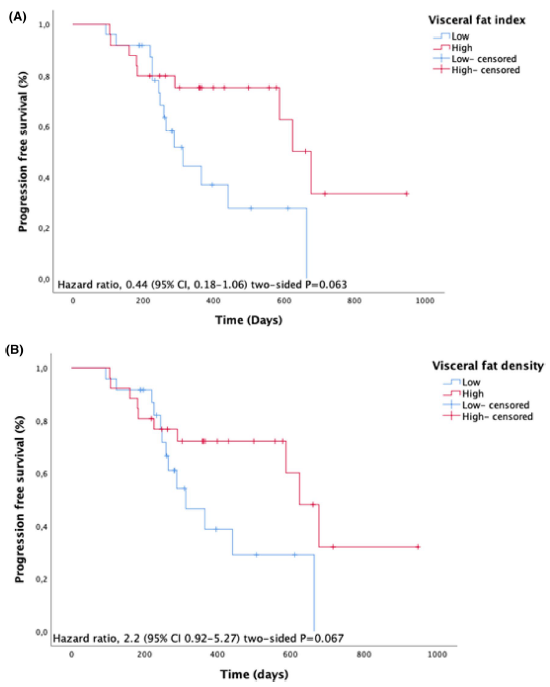
\includegraphics[scale=1.2]{Immagini/franzoi_VAT.png}
\caption{\label{fig:franzoi_VAT} \textit{Diagrammi di Kaplan-Meier della PFS divisi per indice di grasso viscerale alto e basso (A) e densità di grasso viscerale alta e bassa (B). Fonte:} \cite{Franzoi2020}.}
\end{figure}
\begin{figure}[htp]
\centering
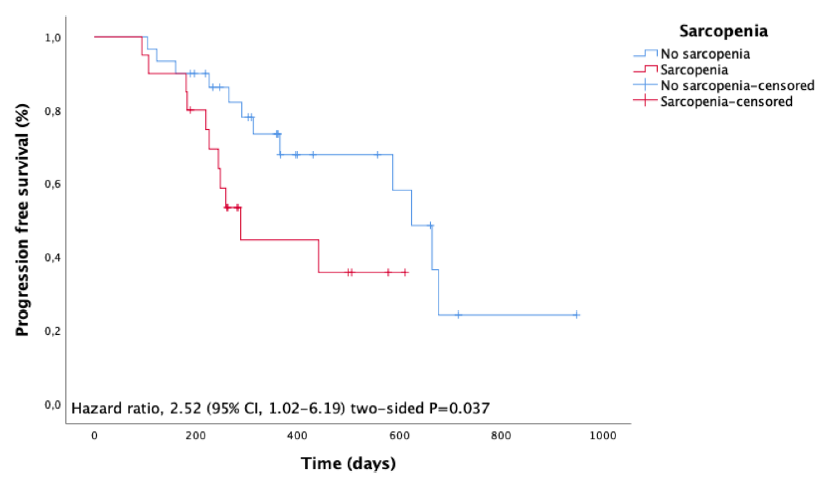
\includegraphics[scale=0.85]{Immagini/franzoi_sarcopenia.png}
\caption{\label{fig:franzoi_sarcopenia} \textit{Diagramma di Kaplan-Meier della PFS diviso in base alla presenza o meno di sarcopenia. Fonte:} \cite{Franzoi2020}.}
\end{figure}

È importante sottolineare che il suddetto effetto protettivo dell'obesità va inteso solo come una maggiore efficacia della terapia a inibitori nei pazienti sovrappeso e obesi rispetto ai pazienti sarcopenici, ma è interessante valutare cosa succede quando le due condizioni si presentano insieme in un paziente, come è stato fatto in un lavoro pionieristico di Prado \textit{et al.} \cite{Prado2008} già nel 2008. Lo scopo di questo lavoro era di accertare la prevalenza e le implicazioni cliniche, in pazienti affetti da carcinomi dei tratti respiratorio e gastrointestinale, dell'obesità sarcopenica, ritenuta a priori dagli autori come il peggior scenario possibile. Il peso e l’altezza dei pazienti sono stati registrati prima dell'inizio della terapia, i pazienti divisi in obesi e non obesi in base al loro BMI e classificati in base al loro stato funzionale, assegnato a ciascun paziente in accordo alle attività fisiche quotidiane riportate dai pazienti stessi. La massa muscolare è stata valutata mediante lo studio di \textit{slice} TC all'altezza della vertebra L3. La coorte iniziale includeva 2115 pazienti di cui il 15\% obesi, sebbene 6 mesi prima della prima misurazione la percentuale di obesi fosse del 27\%, in base alla storia delle variazioni di peso riportata dai pazienti stessi. Dei pazienti classificati come obesi solo 250 disponevano di TC adatte per l’analisi, di cui il 15\% è risultato avere sarcopenia mentre l’85\% no. Sono state trovate differenze significative nell'indice muscolare scheletrico e nella massa magra alipidica tra il campione di pazienti sarcopenici e il campione di pazienti non sarcopenici. L’attenuazione muscolare, misurata in HU, è risultata mediamente inferiore nei pazienti obesi affetti da sarcopenia, il che suggerisce infiltrazioni lipidiche nei muscoli per questa categoria di pazienti. Riguardo alla sopravvivenza, definita in questo caso come il numero di giorni di vita di ciascun paziente dopo la stima del BMI, sono state condotte analisi univariate e multivariate in base ai parametri principali (sesso, età, tipo di cancro, cambiamenti di peso, ecc.) e sono stati eseguiti \textit{log-rank test} per comparare le curve di sopravvivenza in base a ciascun parametro. Il dato più interessante è la comparazione delle curve di sopravvivenza tra pazienti obesi e obesi sarcopenici (\figref{fig:prado_obesitàsarcopenica}), che conferma l'importanza della sarcopenia come indicatore prognostico. Lo studio ha anche trovato indizi sul fatto che la prevalenza dell'obesità sarcopenica possa essere maggiore nei pazienti malati di cancro, sia perché l’obesità è un fattore di rischio per alcuni tipi di cancro, sia perché la sarcopenia è prevalente nei pazienti anziani, così come i tumori.
\begin{figure}[htp]
\centering
\includegraphics[scale=0.65]{Immagini/prado_obesitàsarcopenica.png}
\caption{\label{fig:prado_obesitàsarcopenica} \textit{Diagramma di Kaplan-Meier della sopravvivenza in pazienti obesi e obesi con presenza di sarcopenia. Fonte:} \cite{Prado2008}.}
\end{figure}

Ulteriore conferma all'inadeguatezza del BMI, ma anche della non totale affidabilità dei parametri calcolati mediante tomografia è data dallo studio di Magri \textit{et al.} \cite{Magri2019} sulla correlazione della stima della composizione corporea ottenuta tramite TC e di alcuni parametri metabolici con la sopravvivenza in pazienti affetti da cancro ai polmoni in cura con il nivolumab, un farmaco che stimola la risposta immunitaria contro le cellule tumorali. I parametri confrontati sono il BMI, l’indice di massa muscolare scheletrica (SMI), l’indice di massa magra alipidica (\textit{fat-free mass index}, FFMI), l’indice di massa grassa (FMI), i cambiamenti di peso e il livello di albumina nel sangue. Viene presa in considerazione l’albumina perché è una proteina il cui eccesso è associato a condizioni di malnutrizione o di forte dimagrimento (cachessia). Le misurazioni delle abbondanze dei diversi tessuti è stata effettuata su una singola \textit{slice} a livello della vertebra L3 acquisita con TC non prima di 10 settimane e non dopo 2 mesi rispetto all'inizio dell'immunoterapia. I livelli di albumina sono stati acquisiti non prima di 5 settimane e non dopo 2 settimane rispetto all'inizio dell'immunoterapia. Sorprendentemente, è stato trovato che solo i livelli di albumina e la perdita di peso erano correlati alla sopravvivenza dei pazienti, mentre le grandezze \textit{CT-derived} sono risultate parzialmente correlate con il BMI ma non con l’albumina e con la perdita di peso. Dall'analisi di Kaplan-Meier, gli autori del lavoro hanno trovato una minore sopravvivenza (intesa dall'inizio dell'immunoterapia) nei pazienti che presentavano una perdita di peso superiore al 5\% rispetto agli altri pazienti, e anche una minore sopravvivenza nei pazienti con livelli di albumina nel sangue più bassi del limite inferiore di normalità (\figref{fig:magri_sopravvivenza}). In questo studio, secondo gli autori il primo ad analizzare i cambiamenti di peso nei pazienti durante il primo approccio terapeutico, viene sottolineato per l’appunto il maggior valore prognostico e clinico di una semplice analisi del sangue per la misurazione dei livelli di albumina e del monitoraggio dei cambiamenti di peso rispetto alle grandezze \textit{CT-derived}.
\begin{figure}[htp]
\centering
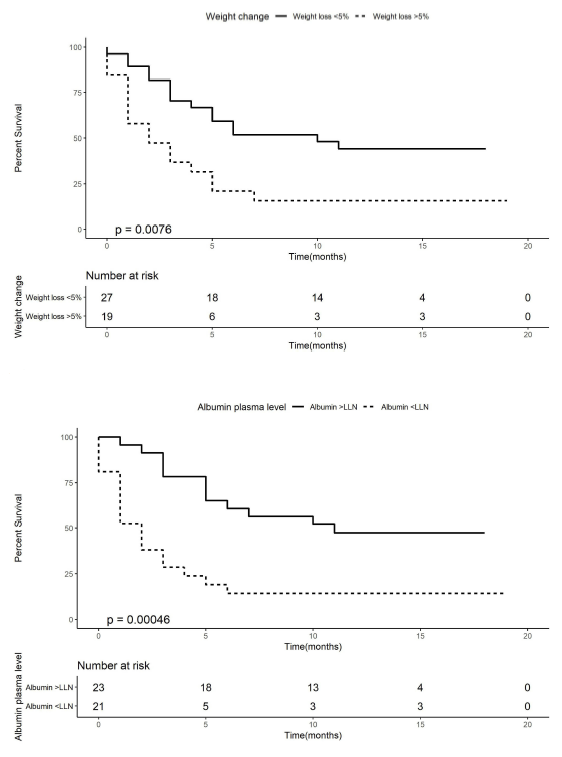
\includegraphics[scale=1.1]{Immagini/magri_sopravvivenza.png}
\caption{\label{fig:magri_sopravvivenza} \textit{Diagrammi di Kaplan-Meier della sopravvivenza divisi per perdita di peso, superiore o inferiore al 5\% (grafico in alto), e livello di albumina, inferiore o superiore rispetto al limite inferiore di normalità (grafico in basso). Fonte:} \cite{Magri2019}.}
\end{figure}

Il monitoraggio dei cambiamenti di peso è fondamentale per la buona riuscita di una terapia antitumorale, fondamentalmente perché la quantità di farmaco da somministrare al paziente si fonda sulla quantità di tessuto adiposo e muscolare. I cambiamenti di peso sono molto frequenti nei pazienti affetti da tumore: innanzitutto la diminuzione del peso senza cambi rilevanti nello stile di vita è uno dei primi campanelli d’allarme per la diagnosi stessa del tumore. In questa fase la diminuzione è causata da alterazioni metaboliche dovute alla risposta del sistema immunitario contro il tumore. Successivamente questo problema può aumentare a causa delle terapie antitumorali, sia la chemioterapia sia la radioterapia, che possono causare riduzione dell'appetito, debolezza muscolare, nausea, vomito e altri effetti collaterali \cite{aimac}. Accanto alla perdita di peso, in risposta ai trattamenti per alcuni tipi di tumori si può avere anche un aumento di peso, anche questo da non sottovalutare. Il caso più eclatante è l’aumento di peso dovuto alla chemioterapia adiuvante per pazienti colpiti da cancro alla mammella. Si tratta di una terapia che viene eseguita comunemente in seguito all'asportazione chirurgica del tumore per aumentare la probabilità di completa guarigione. È stato dimostrato che i pazienti che aumentano di peso più della media con questo tipo di trattamento hanno un maggior rischio di recidive e di morte \cite{Camoriano1990}. Ovviamente la soluzione migliore sarebbe impedire o minimizzare l’aumento di peso ma in ogni caso c’è bisogno di adeguare le cure sulla base della composizione corporea.